\documentclass[12pt]{article}

\usepackage{graphicx}
\usepackage{amsmath}
\usepackage{amsfonts}
\usepackage[style=authoryear, natbib=true, url=false, isbn=false, doi=false, backend=bibtex]{biblatex}
\usepackage[margin=1in]{geometry}
\usepackage[doublespacing]{setspace}

\renewcommand*{\nameyeardelim}{\addcomma\addspace}
\bibliography{ZoteroLibrary}
\renewbibmacro{in:}{}

% arara: pdflatex 
% arara: bibtex 
% arara: pdflatex 
% arara: pdflatex 
\begin{document}

\title{Effective Data Science Education: \\
\large A Project-Based Case Study Perspective}

\author{Daniel Turek$^{*}$, Anthony Suen, Dav Clark}

\date{}

\maketitle

\vspace{0.4in}
\begin{center}

Berkeley Institute for Data Science \\
University of California \\
Berkeley, CA 94720, USA

\vspace{0.8in}

$^*$Corresponding Author \\
dturek@berkeley.edu
\end{center}

\thispagestyle{empty}
\newpage

\begin{abstract}
The discipline of data science has emerged over the past decade as a convergence of high-power computing, data visualization and analysis, and data-driven application domains.  Prominent research institutions and private sector industry have embraced data science, but the foundations for effective tertiary-level data science education are conspicuously absent. This is nothing new, however, as the university has an established tradition of developing its educational mission hand-in-hand with the development of novel methods for human understanding \citep{feingold_tradition_1991}. Thus, it is natural that universities ``figure out" data science concurrent with development of the needed pedagogy. We consider the development of data science education with respect to recent trends in interdisciplinary and experiential educational methodologies, to understand how these apply to data science programs. These perspectives motivate us to consider what factors are necessary to drive effective data science education, which range from a complete end-to-end workflow, technological tools for development and team communications, and appropriate motivation and incentives. The first iteration of the \emph{Berkeley Institute for Data Science (BIDS) Collaborative}, which took place at the University of California, Berkeley in the Spring of 2015, is used as a case study. From this, we draw lessons learned and formulate a hypothesis regarding the necessary components of effective tertiary data science education -- a topic that is presently understudied.  Our hypothesis will be tested and revised in subsequent iterations of the BIDS Collaborative as we continue our study of data science education, research, and social impact.
\end{abstract}

\vspace{0.4in}

\textbf{Keywords:} \\
\indent \indent Data science, Tertiary education, Case study, Experiential learning

\thispagestyle{empty}
\newpage

\section{Introduction}

Owing to the rapid advances in computational power and the on-going ``big data" craze, the discipline of data science has exploded onto the academic and business landscape. Master's programs in data science are now being offered at leading research institutions such as Stanford University and Columbia University, and centers for data science have recently opened their doors at the University of California, Berkeley, the University of Washington, and New York University. Led  by the success of tech giants such as Google, Amazon and Facebook, the increasing availability of data is transforming industries ranging from medicine to media.  The industrial sector is keeping pace by creating and actively recruiting for positions in data science.  The profession of data scientist was even described by the Harvard Business Review as ``the sexiest job of the 21$^{\text{st}}$ century" \citep{Patil2012}.

Despite this inundation of the term ``data science," we still struggle to define what data science is, or to realize any boundaries as to what data science encompasses \citep{Hayashi1998, Loukides2011, Provost2013}. A common Venn diagram places data science squarely at the intersection of computer science, mathematical statistics, and scientific application domains.  This perhaps most accurately reflects that data science is nebulous by nature, having ties to all areas of quantitative scientific research and computational data analysis, but falls short of providing an understanding of how this new discipline will eventually settle into the broader scientific ecosystem.  Fortunately, our aim is not to identify the nature of data science itself, but instead to examine the practicalities and realities of data science education at the tertiary level.

There exists substantial literature regarding best practices and modern approaches to tertiary education. This has been a subject of interest since the first modern universities appeared in Europe in the sixteenth century \citep{Rudy1984, Pedersen1997}.  Since then, modern approaches to higher education have evolved immensely due to advances in technology, and also society's attitude towards higher education.  Perhaps the single most transformative influence on higher education has been the so-called digital revolution of the past few decades, which has had a profound impact on the content and style of tertiary education \citep{Roberts1994, Ely1995, Baker1997, Wood2005, Baek2008}.

Some research suggests that traditional approaches to tertiary education may only result in superficial learning, rather than a deep understanding of subject material \citep{Entwistle1992}.  Thus, the study of education itself is an area of prime interest.  Many approaches have been suggested and studied over the past decades, attempting to improve the quality of tertiary education.  \citet{Topping1996} promotes the practice of peer tutoring, while others have more recently endorsed ``flipped classrooms" in which learning is self-directed rather than instructor-directed, and classrooms become a place for practice instead of lecture \citep{Horn2013, Herreid2013}.  \citet{Ogawa1995} suggests a ``mutiscience" approach to multidisciplinary science education, in which the diversity scientific disciplines is recognized and incorporated into the educational system.  The approach of ``constructive alignment" provides one example of outcome-based education, in which teaching and assessments are constructed to align with the desired educational outcomes \citep{biggs2003aligning, biggs2011teaching}.  And the frequently utilized approach of project-based learning has now been promoted at the institutional level for many years \citep{Thomas2000, Krajcik2006}.

The focus of our analysis is specifically the education of data science. In light of the academic and industrial spotlight on data science, the best practices for data science education should be an active area of research, just as it is for tertiary education in general.  However, owing to its relatively recent mainstream debut, there is an absence of scientific research or published literature in this area.  Furthermore, there exists no widely-accepted model for scalable project-based data science education, the existence of which would have a profound impact at the tertiary level.  These facts motivate our analysis of the history, current trends, and future prospects of data science education.

We aim to begin filling this void by analyzing a tangible case study of data science education, which was undertaken at the University of California, Berkeley, under the name of the BIDS Collaborative. We consider the successes and failures of the first cohort to pass through the BIDS Collaborative, and the pain points which were encountered by the students and Collaborative facilitators, alike.  We make practical recommendations for educational approaches to data science curricula, and formulate a hypothesis regarding the best practices of tertiary data science education.  Study of our hypothesis will require subsequent experiential testing, which will be the subject of future research.



\section{Paradigms of Science Education}

To set the context for data science training and research methods, we review two educational paradigms that have become prominent in recent decades. These are the interdisciplinary research and the experiential learning educational models.  As we describe these educational paradigms, we also discuss how they drive the practices employed by the BIDS Collaborative.

\subsection{Interdisciplinary Research}

Interdisciplinary or multidisciplinary research is ``a format for conversation and connections that will lead to new knowledge" \citep{repko2008interdisciplinary}. This word has been a fashionable academic buzzword for several decades, but the approach of looking at and solving issues from multiple angles has failed to fundamentally scale beyond the confines of certain research groups to change the manner in which research is conducted. There are major obstacles such as cultural, organizational, and technical barriers that prevent the effectiveness of such learning and research environments \citep{eisenberg2000bridging}.

Genuine interdisciplinary training is not generally taught as would be practically necessary.  This lack of training is due in part to university organizational structures, with departments providing little or no incentives for interdisciplinary collaborations. As jobs prospects for those who genuinely have a multidisciplinary focus are usually inferior, it creates a self-propagating cycle that reinforces single disciplinary specialist work. 

These organizational structures also create silos surrounding sets of technical tools.  Different software and methods are used to achieve similar goals via widely divergent means, potentially obscuring the fact that disparate groups are in fact grappling with the same underlying problems. Social scientists, the physical sciences, and areas of engineering use distinct sets of tools to address data, despite using models that often have similar predictive goals. For example, Stata \citep{stata2005stata} might be used by an economist, Matlab \citep{incorporation2005matlab} by the engineer, and R \citep{RCoreTeam2014} by the statistician. This divergence and specialization in tools creates an ever widening gap between major disciplines.  These pose obstacles to true interdisciplinary collaboration among diverse teams of researchers.

Observing these barriers to multidisciplinary data science, the approach of the BIDS Collaborative was two-fold. First, it implemented a framework for interdisciplinary learning beyond traditional academic lecture and coursework structures. Second, it cultivated an environment independent of the traditionally established incentive structure of academic departments. The goal of this novel approach was to demonstrate that interdisciplinary research was possible with limited resources and incentives, and that data science tools can be readily shared across disciplines.

This mission highlights the need for a particular style of leadership within multidisciplinary teams.  The Collaborative hypothesized this style of leadership might exist more naturally among student teams than among academic faculty, on account of having lower barriers towards new technology and incentive structures, and generally a stronger feeling of openness to approaching problems in a new way.  Collaborative facilitators believed that multidisciplinary collaboration would be easier when the stakes are lower than among traditional academic faculty, and learning takes place within student peer groups.

\subsection{Experiential Learning (Flipped Classroom)}

The Collaborative supported its interdisciplinary mission with projects that were genuinely experientially focused.  This involved external clients and real-world data. Under this model, students no longer played passive roles in the educational process, but instead their active participation drove the educational mechanism \citep{beard2010experiential}. Instead of teachers transmitting knowledge, mentors and facilitators ensured that projects and learning were on track, and that needed resources were available. This model for education is also known as a flipped classroom \citep{Horn2013}.

Research from Stanford University \citep{plotnikoff_classes_2013} has validated that flipped classroom experiential learning is a stronger learning strategy compared to the traditional approach of combining lectures and homework. Requiting students to actively contribute has been shown to be effective in accelerating knowledge acquisition. This experiential approach means removing the traditional framework of lectures and tests entirely. 

Experiential learning also emphasizes project management, since traditional classroom assignments have clear deadlines imposed by the professor \citep{mok2014teaching}. Given the diverse nature of data science projects, limited staffing resources, and the need to manage relationships with clients, the Collaborative facilitators believe that students must assume roles as project managers.  As an added benefit, the experiential learning approach is also a more realistic representation of practical data science in the real world.



\section{Case Study: BIDS Collaborative}

The first iteration of the BIDS Collaborative was carried out at the Berkeley Institute for Data Science, in the Spring semester of 2015.  The central principle of the Collaborative was to organize teams of student researchers around real-world data science projects. In applied data science, project domains and materials must be relevant to researcher backgrounds. Thus, a primary concern was to provide projects that would be of interest to a wide variety of students.  Collaborative facilitators initially collected a diverse set of 16 projects from a wide variety of organizations.

We first describe the projects which made up the first iteration of the BIDS Collaborative.  Next, we detail of the process of project selection and team formation which ultimately resulted in these research project teams.  We describe the most commonly used tools, and present the temporal workflow pattern of each team.  Finally, we related these diverse workflows to the successes and challenges that teams experienced throughout the semester.

\subsection{Projects}

The first iteration of the BIDS Collaborative ran four data science research projects.  The client organizations backing these projects represented both industry and academia.  We first present a short description of each project.

\subsubsection*{DeStress: Text Mining for Stress}

This was one of two projects that was driven by Berkeley faculty involvement. What differentiated this project from traditional faculty-driven research was the inclusive call for participation, and the engagement in a collaborative open-source development framework. This project pursued Professor of Computer Science John Canny's BIDMach system (\texttt{http://bid2.berkeley.edu/bid-data-project/}; \cite{canny2013bidmach}), which is a performant GPU-accelerated system for machine learning in the Scala language. A domain focus on determining stress and major life events using large scale machine learning was chosen by one of Professor Canny's graduate students.

The project was enabled in part by providing a commodity workstation that was already available in the Berkeley D-Lab (\texttt{http://dlab.berkeley.edu/}), with the addition 1TB of hard disk storage. Thus, while this project was at the boundrary of machine learning, the resources for this project would be readily accessible to modestly funded labs.  The DeStress project and code is available at \texttt{https://github.com/berkeley-dsc/destress}.

\subsubsection*{Underclub: Online Business Survey Feedback}

While intention of the Collaborative was to primarily recruit clients from outside the university, Underclub was ultimately the only client that approximated this intent. Indeed, even they had a pre-existing affiliation with the University through Berkeley's Haas school of business.  In this project, students analyzed survey response data from a start-up company centered around online clothing distribution and sales.  Using this data, recommendations were made for the business client regarding how to appropriately address market segmentation and the inherent challenges of online marketplaces.  Given the business-related nature of this work, it was carried out in a private online repository.

\subsubsection*{Finance: Analyzing Financial Market Data with Apache Spark}

The Finance project was the second of two that was driven by a member of the Berkeley faculty; in this case Professor of Law Justin McCrary, who also serves as the faculty director of the Berkeley D-Lab. Professor McCrary's research includes the development efficient workflows to take advantage of the Berkeley campus compute cluster, Savio. To this end, this project worked with the Berkeley Research Computing team that manages the Savio cluster to enable a modern workflow using Apache Spark (\texttt{http://spark.apache.org/}).

This project was likely of the highest value to campus, as it improved the ability to take advantage of the impressive parallel capabilities that are now provided to all senior campus researchers -- particularly for those users who may need something other than a traditional high performance computing workflow. This code was maintained and organized at \texttt{https://github.com/berkeley-dsc/dlab-finance}.

\subsubsection*{Purchasing: University of California Berkeley Strategic Sourcing}

The director of the University of California's Strategic Sourcing Unit had a pre-existing connection with the Berkeley D-Lab, through use of D-Lab python training and consulting services. This work led to a talk at the SciPy 2014 conference discussing how straightforward scientific python scripts could accelerate previously spreadsheet-based analyses. A Collaborative facilitator assisted in this work, and was therefore aware of the possibilities to save the Strategic Sourcing Unit time and money. From the perspective of an academic institution, this project illustrates an exciting double-win, with potential benefits both to Berkeley administration and student training.  The project was organized at \texttt{https://github.com/berkeley-dsc/purchasing}.

\subsection{Team Formation and Leadership}

Team formation was somewhat chaotic and arguably the most difficult part of the process from the perspective of Collaborative facilitators.  Prospective participants were attracted via two informational sessions held at the beginning of the semester, each of which consisted of an introductory presentation and project pitches.  As may be clear in hindsight, student enthusiasm for projects was driven almost entirely by the physical presence of a client to deliver the project pitch.

Afterwards, students were encouraged to mingle and discuss their research interests, and to self-organize into teams around the available projects. Towards this end, facilitators provided an editable online spreadsheet for team organization. While self-organization might work more efficiently via a system that could enforce a set of rules and policies, allowing all students to collaboratively edit a spreadsheet created numerous problems. The most dramatic difficulty occurred when a large number of student responses were inadvertently deleted from the spreadsheet.

Ultimately, the efforts to provide a self-service organizational approach required facilitators to engage in a time-intensive process of organizing teams via extensive conversations in person and via email. While attendance at the mixers was quite strong, the Collaborative initially retained sixteen individuals with an additional three joining several weeks into the semester. One individual subsequently dropped out mid-semester, though participation was otherwise stable.  The final project teams consisted of between four and six members, with team members representing a variety of academic disciplines.  

An additional challenge at the beginning of the semester was the lack of well-established team leadership. Teams could best be described as loose assemblies of individuals working largely independently on a common project, and progress was slow. Recognizing this lack of cohesion, the Collaborative facilitators suggested that each team choose a lead.  Generally, a single student from each team volunteered to assume this role. Some students openly expressed their reluctance to engage in team leadership, as their interest was primarily in hands-on experience.  Thereafter, team leads exercised some degree of authority in directing projects, delegating responsibilities, and organizing team meetings.  To be clear, the concept of authority was very gently exercised.  Team leads also related current progress and intended future work to Collaborative facilitators.

\subsection{Tools and Workspace}

While team participants were initially divided on the issue, all teams quickly adopted GitHub (\texttt{https://github.com/}; \cite{dabbish2012social}) for collaborative development.  Teams formed in mid-February, and all teams were committing to GitHub by March, concurrent with training sessions provided in the use of collaborative tools.  At the suggestion of Collaborative facilitators, a subset of project teams also adopted Slack for intra-team communications.  Otherwise, teams exhibited significant variation in the tools used for data management, scientific computing, visualizations, and even the final presentation of results.

Teams were allowed unrestricted access to the workspace and conference facilities of the Berkeley Institute for Data Science.  The usage of communal working space within BIDS was initially ad hoc, and some members of the larger BIDS community found this unstructured usage to be disruptive. This was addressed by identifying a particular weekday when Collaborative participants were encouraged to fully utilize the BIDS space -- and to be particularly respectful outside of this time.

\subsection{Workflows}

Each project followed a somewhat idiosyncratic course through the semester-long undertaking, although there were clear commonalities in terms of challenges and solutions.  The GitHub usage commit history of each team is shown in Figure~\ref{fig:gitcommits}, the data for which is publicly available at individual project websites.  These GitHub commit histories are presented alongside the project management workflow employed by the Collaborative facilitators, and the research workflows that project teams were encouraged to follow.

\begin{figure*}[h]
\centerline{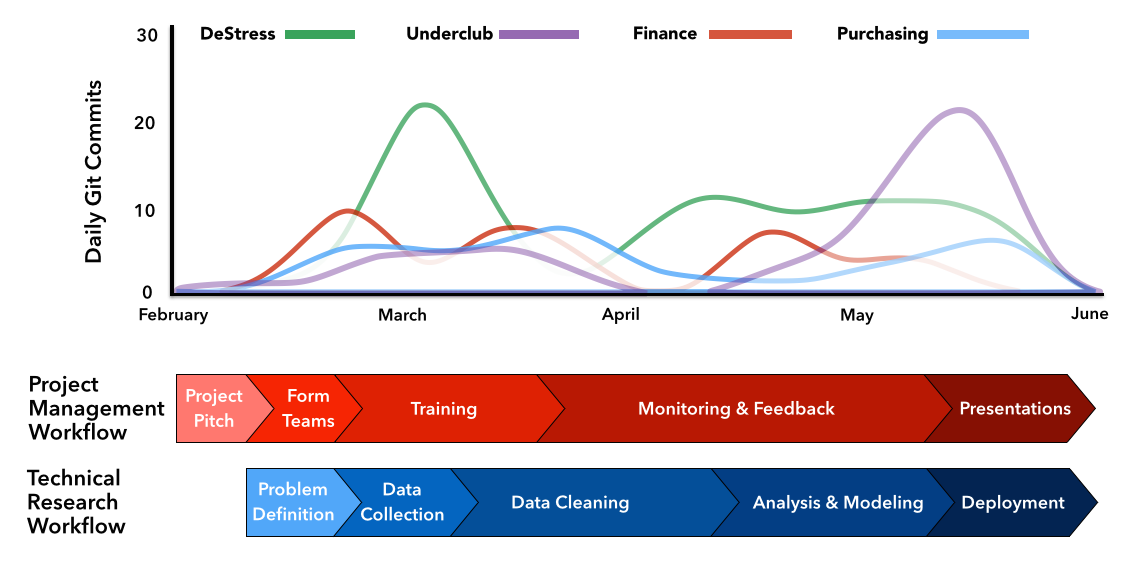
\includegraphics[scale=0.435]{BIDS_Collaborative_Workflow_NEW.png}}
\caption{GitHub commit histories of BIDS Collaborative teams overlaid with project management and technical research workflows.}
\label{fig:gitcommits}
\end{figure*}


This DeStress project maintained robust activity throughout the semester, perhaps exemplifying the ideal project workflow.  Team members were especially active during the early training sessions, coinciding with their data collection and data cleaning work.  This placed the team in a strong position for the remainder of the semester, where members were competent in the usage of tools and well-prepared for the analysis and modeling phase.  This project produced excellent technical research and final presentation, and the participants are currently working towards several publications resulting from this work.

Underclub participants struggled in the early stages, and team members lagged in adopting the collaborative tools.  As a result this project produced few actionable insights, as was apparent in their final presentation -- although some promising directions were established. It is clear that more guidance was needed to efficiently connect their analyses with potential business-relevant actions.  A further shortcoming of the Underclub project was the failure to create a public repository, which would serve as a public record of team progress. This is somewhat understandable, however, given the relatively short timeframe of a single academic semester.  Some efforts were made at the conclusion of this project to create open version of the work for public consumption, as is indicated by the final push through the deployment phase.

Unlike other projects, the Finance project suffered from non-trivial startup overhead.  This included software installation challenges, and integration with the traditional high performance computing scheduler. As such, much of the semester was spent attaining proof-of-concept workflows using Spark to analyze a subset of the full dataset.  Having achieved this proof-of-concept, the Finance project has led to continued work in the Berkeley D-Lab, though primarily with a different set of contributors. This transition underscores the value of working in public repositories for genuinely open-ended projects, where new contributors can pick up where previous efforts left off.

The Purchasing project demonstrated the difficulties for a team of graduate students to undertake a meaningful research project, when working only a few hours per week throughout the semester.  Team activity and progress were slow throughout the course of the Collaborative.  Some progress was made, however, in identifying basic workflows and determining which questions appear to be answerable. In particular, clustering techniques showed promise in identifying subtle partnerships, where collective purchasing could result in savings.  As a result of modest efforts, this project produced a minimal set of useful results.



\section{Lessons Learned}

The first iteration of the BIDS Collaborative was an experimental undertaking, in which both participants and Collaborative facilitators were forging new ground and learning throughout the process.  The Collaborative experienced both successes and failures, and many lessons for effective data science education became apparent.  These lessons have been documented, and will serve as guidance for subsequent iterations of the Collaborative. These lessons help motivate our final hypothesis addressing the ingredients necessary for effective data science education.

\subsection{Project Vetting}

Using a model where students select among pre-determined projects, it is important to present options representing a broad variety of disciplines.  For example, this includes having projects relating to physical sciences, social sciences, technology, health, environment, commerce, among other possibilities.  The Collaborative was very successful in this manner.  By presenting this diverse range of project options, it leveraged students' innate interests in particular areas of study; thus, students were not shoehorned into a research area of little or no interest to them.

The careful framing and acquisition of data for projects was necessary for project success.  Specifically, the logistics of each project must be fully in order and have a well-defined goal.  Only projects fitting this mold were adopted by students in the Collaborative, while other projects languished.  This extended to having a responsive and dedicated individual representing the backing client organization.  And most importantly, the relevant data must be available in advance, such that students could get a sense of the project and could begin work immediately.  This consideration also encompasses any legal releases or non-disclosure agreements pertaining to data access.

\subsection{Team Formation and Leadership}

The Collaborative was largely unsuccessful in the initial organizational process of project teams.  This led to a difficult first month both for participants and facilitators.  We conclude that project and team components must be organized in the appropriate order.  This should begin by identifying clients with data science research projects of the appropriate scale.  The next step is to identify student team leads who are capable of leading a research team and interacting with the client.  Once this organization in place, it is possible to assemble team members for each project based on students' interests and skill sets.  We conclude that only by following this order of \emph{project client, data, team lead, team members}, will each step flow smoothly in succession.

The subsequent iteration of the Collaborative will utilize this lesson and identify upfront team leads for each project.  At this point, facilitators can work with team leads to select remaining team members. This will serve to simplify and distribute the process of team formation, while also clearly establishing a leadership role for the team lead from the onset of each project.

It was apparent that regular interactions between clients and team leads was necessary. Team leads served as the bridge for processing and presenting the client needs to team members.  It was not possible for the Collaborative facilitators to fill this role.  It was impractical to micro-manage each project at this level, and requiring this direct interaction between clients and team leads allowed students to self-organize, providing the reality of undertaking real-world research projects.  This approach provided a sense of responsibility and accomplishment for team leaders and team members.

\subsection{Milestones}

The Collaborative was successful at creating well-defined intermediate goals, which helped maintain team momentum throughout the semester.  These goals took for the form of data-centric milestones, such as data cleaning or preliminary data exploration.  Formally assigning dates for these milestones ensured forward progress.  In addition, this helped the Collaborative facilitators passively monitor the progress of individual teams, and provide additional help when necessary.  Larger milestones included a mid-semester presentation, and a capstone evening event including final presentations to client organizations.  We consider these milestones as being critical to the short-term nature of education spanning a single academic semester.

\subsection{Training and Tools}

The Collaborative was not entirely successful at the early introduction and promotion of collaborative tools.  The most successful project teams immediately adopted GitHub for all project code and Slack for team communications.  It appeared that the sooner team members adopted these tools into their research workflows, the sooner meaningful progress began.  We conclude it is critical to introduce these tools to students early, and promote, if not mandate their usage for teamwork and communications.

The upcoming iteration of the Collaborative will adopt a clear plan for the beginning of the semester. Students will attend a weekly practicum that will include orientations to technical tools, collaborative tools, and project management and documentation.



\section{Closing}

A number of open questions remain from the first iteration of the BIDS Collaborative.  We discuss several of these questions, then present our conclusions and hypothesis for the future of data science education.

\subsection{Open Questions}

The Collaborative explored the possibility of offering Berkeley academic credit as motivation for student engagement, but no students pursued this option. It is unclear why this was not an effective motivational tool, although it may be due to the absence of a time-tested process and the presence of additional bureaucratic hurdles. An alternative approach could be creating an integrated framework with an existing project-based course, which will be explored for the next iteration of the Collaborative.  Even so, the option of receiving academic credit did not appear to be a strong motivator for students.

Some students, however motivated, were not technically prepared for jumping into a data science research project.  This drives the need to provide early technical training sessions.  However, the best approach to scheduling, the precise material, and the optimal frequency of these training sessions remains an open question.  Furthermore, it is debatable whether student attendance should be compulsory, since mandating attendance may begrudge technically-savvy students.  Training could potentially overlap with existing campus workshop or training programs.  This would conserve Collaborative resources and provide scalability, but would also dictate the scheduling, frequency, and material.

The best approaches to managing and motivating teams remains an open topic of discussion.  One approach is to micro-manage individual project teams, and have facilitators attend regular weekly team meetings.  However, this level of management is extremely time-consuming and not scalable, and furthermore, not always appreciated by student groups.  Similarly, how to motivate a semester-long commitment from participants is a difficult question.  Fundamentally, the Collaborative would like to rely on students' desires for real-world data science experience, but this is a lofty goal and may not always suffice.  The best motivational approaches are yet unclear, and exactly which techniques prove successful will be an area of scrutiny throughout the next Collaborative.

\subsection{Conclusions}

The BIDS Collaborative was an educational experiment in data science education, executed with bare bones staffing and support. Despite lacking the resources typical of traditional university educational programs, it was nonetheless successful in motivating a group of students to undertake real-world data science projects over the course of an academic semester.  The design and overall success of the BIDS Collaborative program shows promise in terms of scalability to the larger university level.

The first iteration of the Collaborative brought a variety of practical considerations for effective data science education to light.  Perhaps foremost is the importance of having real-world projects drawn from interested client organizations, and are backed by accessible data, ready at hand.  Forethought about the relationships and communication lines between clients, projects team leads, and team members also proved to be surprisingly important for the smooth operation of the research teams.  Finally, the early introduction and training of the appropriate technical and collaborative tools was also seen to be necessary for effective team research.

We hypothesize that effective multidisciplinary data science education must address the complexities which are fundamental to both technical research and human team dynamics. This requires imposing a structured hierarchy for client-team dynamics, augmented with workshops and consulting services to provide the resources necessary for productive research.  Most importantly, we note the value of a real-world capstone collaborative project which provides genuinely experiential learning, which we feel is a critical component of effective data science education.

Stepping back, we have suggested best practices for successfully organizing and motivating multidisciplinary teams to solve real-world data-centric challenges.  Although these lessons arose from a semester-long program for experiential data science education, they apply equally well to experiential learning in other disciplines.  We believe our general conclusions may benefit project-based educational programs throughout university systems as a whole.



\newpage

%\bibliographystyle{apa}
%\bibliography{ZoteroLibrary}

\newpage
\printbibliography

\end{document}





